\documentclass[12pt]{article}
\usepackage[utf8]{inputenc}

\usepackage{lmodern}

\usepackage{enumitem}
\usepackage[margin=2cm]{geometry}

\usepackage{amsmath, amsfonts, amssymb}
\usepackage{graphicx}
%\usepackage{subfigure}
\usepackage{tikz}
\usepackage{pgfplots}
\usepackage{multicol}

\usepackage{comment}
\usepackage{url}
\usepackage{calc}
\usepackage{subcaption}
\usepackage[indent=0pt]{parskip}
\usepackage{animate}

\usepackage{array}
\usepackage{blkarray,booktabs, bigstrut}
\usepackage{bigints}

\pgfplotsset{compat=1.16}

% MATH commands
\newcommand{\ga}{\left\langle}
\newcommand{\da}{\right\rangle}
\newcommand{\oa}{\left\lbrace}
\newcommand{\fa}{\right\rbrace}
\newcommand{\oc}{\left[}
\newcommand{\fc}{\right]}
\newcommand{\op}{\left(}
\newcommand{\fp}{\right)}

\newcommand{\bi}{\mathbf{i}}
\newcommand{\bj}{\mathbf{j}}
\newcommand{\bk}{\mathbf{k}}
\newcommand{\bF}{\mathbf{F}}

\newcommand{\mR}{\mathbb{R}}

\newcommand{\ra}{\rightarrow}
\newcommand{\Ra}{\Rightarrow}

\newcommand{\sech}{\mathrm{sech}\,}
\newcommand{\csch}{\mathrm{csch}\,}
\newcommand{\curl}{\mathrm{curl}\,}
\newcommand{\dive}{\mathrm{div}\,}

\newcommand{\ve}{\varepsilon}
\newcommand{\spc}{\vspace*{0.5cm}}

\DeclareMathOperator{\Ran}{Ran}
\DeclareMathOperator{\Dom}{Dom}

\newcommand{\exo}[1]{\noindent\textcolor{red}{\fbox{\textbf{Problem {#1}}}\hrulefill}\\\\ }
\newcommand{\qu}[4]{\noindent\textcolor{#4}{\fbox{\textbf{Section {#1} | Problem {#2}}} \hrulefill{{\fbox{\textbf{{#3} Points}}}}\\}}

\newcommand{\semester}{Fall 2023}

\newcommand{\CVup}{%

\begin{tikzpicture}
\draw[black, <->, >=latex] (-0.33, 0.5) .. controls (-0.125, 0) and (0.125, 0) .. (0.33, 0.5);
\end{tikzpicture}}

\newcommand{\CVupInc}{%
\begin{tikzpicture}
\draw[black, ->, >=latex] (0,0) .. controls (0.2, 0) and (0.4, 0.2) .. (0.5, 0.5);
\end{tikzpicture}}

\newcommand{\CVupDec}{%
\begin{tikzpicture}[rotate=270]
\draw[black, ->, >=latex] (0,0) .. controls (0.2, 0) and (0.4, 0.2) .. (0.5, 0.5);
\end{tikzpicture}}

\newcommand{\CVdown}{%
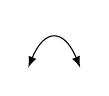
\begin{tikzpicture}
\draw[black, <->, >=latex] (-0.33, -0.5) .. controls (-0.125, 0) and (0.125, 0) .. (0.33, -0.5);
\end{tikzpicture}}

\newcommand{\CVdownInc}{%
\begin{tikzpicture}
\draw[black, ->, >=latex] (-0.5, -0.5) .. controls (-0.5, -0.3) and (-0.5, -0.1) .. (0,0);
\end{tikzpicture}}

\newcommand{\CVdownDec}{%
\begin{tikzpicture}[rotate=-90]
\draw[black, ->, >=latex] (-0.5, -0.5) .. controls (-0.5, -0.3) and (-0.5, -0.1) .. (0,0);
\end{tikzpicture}}

\begin{document}
	\noindent \hrulefill \\
	MATH-244 \semester \hfill Practice Problems Solutions\\
	Section 15.2 \hfill Pierre-Olivier Paris{\'e} \\\vspace*{-1cm}
	
	\noindent\hrulefill
	
	\spc	

	\exo{6}
	\\
	We first have that
		\begin{align*}
		\int_0^{e^v} \sqrt{1 + e^v} \, dw = \sqrt{1 + e^v} \left. \left( w \right) \right|_{0}^{e^v} = e^v \sqrt{1 + e^v} .
		\end{align*}
	So
		\begin{align*}
		\int_0^1 \int_0^{e^v} \sqrt{1 + e^v} \, dw dv = \int_0^1 e^v \sqrt{1 + e^v} \, dv = \frac{2}{3} ( (1 + e)^{3/2} - 2 \sqrt{2} ) \approx 2.894 .
		\end{align*}
	
	\spc
	
	\exo{14}
	\\
	The first thing to do is to draw the region $D$.
	
		\begin{figure}[h]
		\centering
		\includegraphics[scale=0.3]{sketch-exo14-Domain.png}
		\end{figure}
	We see that the curves $y = x^2$ and $y = 3x$ intersects at the points $(0,0)$ and $(3, 9)$.
	
	\begin{enumerate}
	\item[\textbf{Type I}] We have $0 \leq x \leq 3$ and $x^2 \leq y \leq 3x$. So the functions bounding the values of $y$ are $x^2$ and $3x$. As a type I, the domain is written as
		\begin{align*}
		D = \{ (x, y) \, : \, 0 \leq x \leq 2 \text{, } x^2 \leq y \leq 3x \} .
		\end{align*}
	\item[\textbf{Type II}] We see that $0 \leq y \leq 9$ and since $x \geq 0$, the curves bounding the values of $x$ are $x = y/3$ and $x = \sqrt{y}$. As a a type II, the domain is written as
		\begin{align*}
		D = \{ (x, y) \, : \, y/3 \leq x \leq \sqrt{y} \text{, } 0 \leq y \leq 9 \} .
		\end{align*}
	\end{enumerate}
	Now the integral is
		\begin{align*}
		\int_0^3 \int_{x^2}^{3x} xy \, dy dx = \int_0^3 x \Big(\frac{9x^2 - x^4}{2}\Big) \, dx = \int_0^3 \frac{9x^3 - x^5}{2} = \frac{243}{8} .
		\end{align*}
	If you chose the other way, then your integral should look like this:
		\begin{align*}
		\int_0^9 \int_{y/3}^{\sqrt{y}} xy \, dx dy .
		\end{align*}
		
	\spc
		
	\exo{30}
	\\
	The solid we are trying to find the volume is represented in the figure below.
	\begin{figure}[h]
	\centering
	\includegraphics[scale=0.4]{sketchExo30.png}
	\includegraphics[scale=0.4]{sketchExo30-Solid.png}
	\end{figure}
	
	To find the domain of integration $D$, we have to project the surfaces $y^2 + z^2 = 4$ and $x = 2y$ on the $XY$-place. For the first surface, we obtain $y = \pm 2$ (two horizontal lines in the $XY$-plane) and $x = 2y$ (a line with slope $1/2$). So the domain of integration is the following region:
	\begin{figure}[h]
	\centering
	\includegraphics[scale=0.2]{sketch-Exo30_Domain.png}
	\end{figure}
	So, the domain $D$ is
		\begin{align*}
		D = \{ (x, y) \, : \, 0 \leq x \leq 2y \text{, } 0 \leq y \leq 2 \} .
		\end{align*}
	
	The function to integrate is $z = \sqrt{4 - y^2}$. Thus, the volume of the solid $S$ is given by
		\begin{align*}
		V (S) = \int_0^2 \int_{0}^2y \sqrt{4 - y^2} \, dx dy = \int_0^2 2y\sqrt{4 - y^2} \, dy .
		\end{align*}
	The integral with $2y \sqrt{4 - y^2} \, dy$ is done by a change of variable and we get
		\begin{align*}
		\int_0^2 2y \sqrt{4 - y^2} \, dy = \frac{16}{3} .
		\end{align*}
	Thus, the volume of the solid is
		\begin{align*}
		V (S) = \frac{16}{3} .
		\end{align*}
	
	\spc
	
	\exo{52}
	\\
	From the limits in the integrals, we see that $0 \leq x \leq 1$ and that $x^2 \leq y \leq 1$. So the region of integration looks like this:
		\begin{figure}[h]
		\centering
		\includegraphics[scale=0.3]{exo-HW02.png}
		\end{figure}
	So the region $D$ is the region bounded by the curves $x = 0$, $y = x^2$, and $y= 1$. Since $x \geq 0$, the region $D$ is also the region bounded by the curves $x = 0$, $x = \sqrt{y}$, and $y = 1$. So we can say that
		\begin{align*}
		D = \{ (x, y) \, : \, 0 \leq x \leq \sqrt{y} , 0 \leq y \leq 1 \} .
		\end{align*}	
	Thus, the integral now becomes
		\begin{align*}
		\int_0^1 \int_0^{\sqrt{y}} \sqrt{y} \sin y \, dx dy = \int_0^1 \sqrt{y} \sin (y) \Big( \sqrt{y} - 0 \Big) \, dy = \int_0^1 y \sin y \, dy .
		\end{align*}	
	After an integration by parts, we get the value of the integral:
		\begin{align*}
		\int_0^1 \int_0^{\sqrt{y}} \sqrt{y} \sin y \, dx dy = \sin (1) - \cos (1) \approx 0.301168
		\end{align*}			

\end{document}